%--- Select slide document and theme ---%
\documentclass{beamer}
\usetheme{Madrid}

%--- Swedish support ---%
\usepackage[T1]{fontenc}      
\usepackage[swedish]{babel}
\usepackage[latin1]{inputenc}

%--- verbatim support ---%
\usepackage{verbatim}
\newenvironment{VerbExample}
{\example\semiverbatim}
{\endsemiverbatim\endexample}


%--- Graphics ---%
\usepackage{graphicx}

%--- Label itemize blocks ---%
\usepackage{enumitem}


\begin{document}
\title{FRTN01 project - Group 20}
\subtitle{Control of Batch Tank using Raspberry Pi}
\author{Johan Anderholm \\ Jonathan Kämpe \\ Mikael Sahlström \\ Mikael Nilsson}
\institute[LTH]{LTH}
\date{\today}

%--- the titlepage frame -------------------------%
\begin{frame}[plain]
  \titlepage
\end{frame}

%--- Slide 1 ---%
\begin{frame}{Project description}
\begin{columns}[T]
    \begin{column}{.55\textwidth}
        \begin{itemize}
            \item In pump to control the temperature.
            \item Out pump to control the water level.
            \item Heater to simulate the exothermic process.
            \item Cooler.
            \item Mixer.
        \end{itemize}
    \end{column}
    \begin{column}{.45\textwidth}

        \begin{figure}[H]
           \centering
           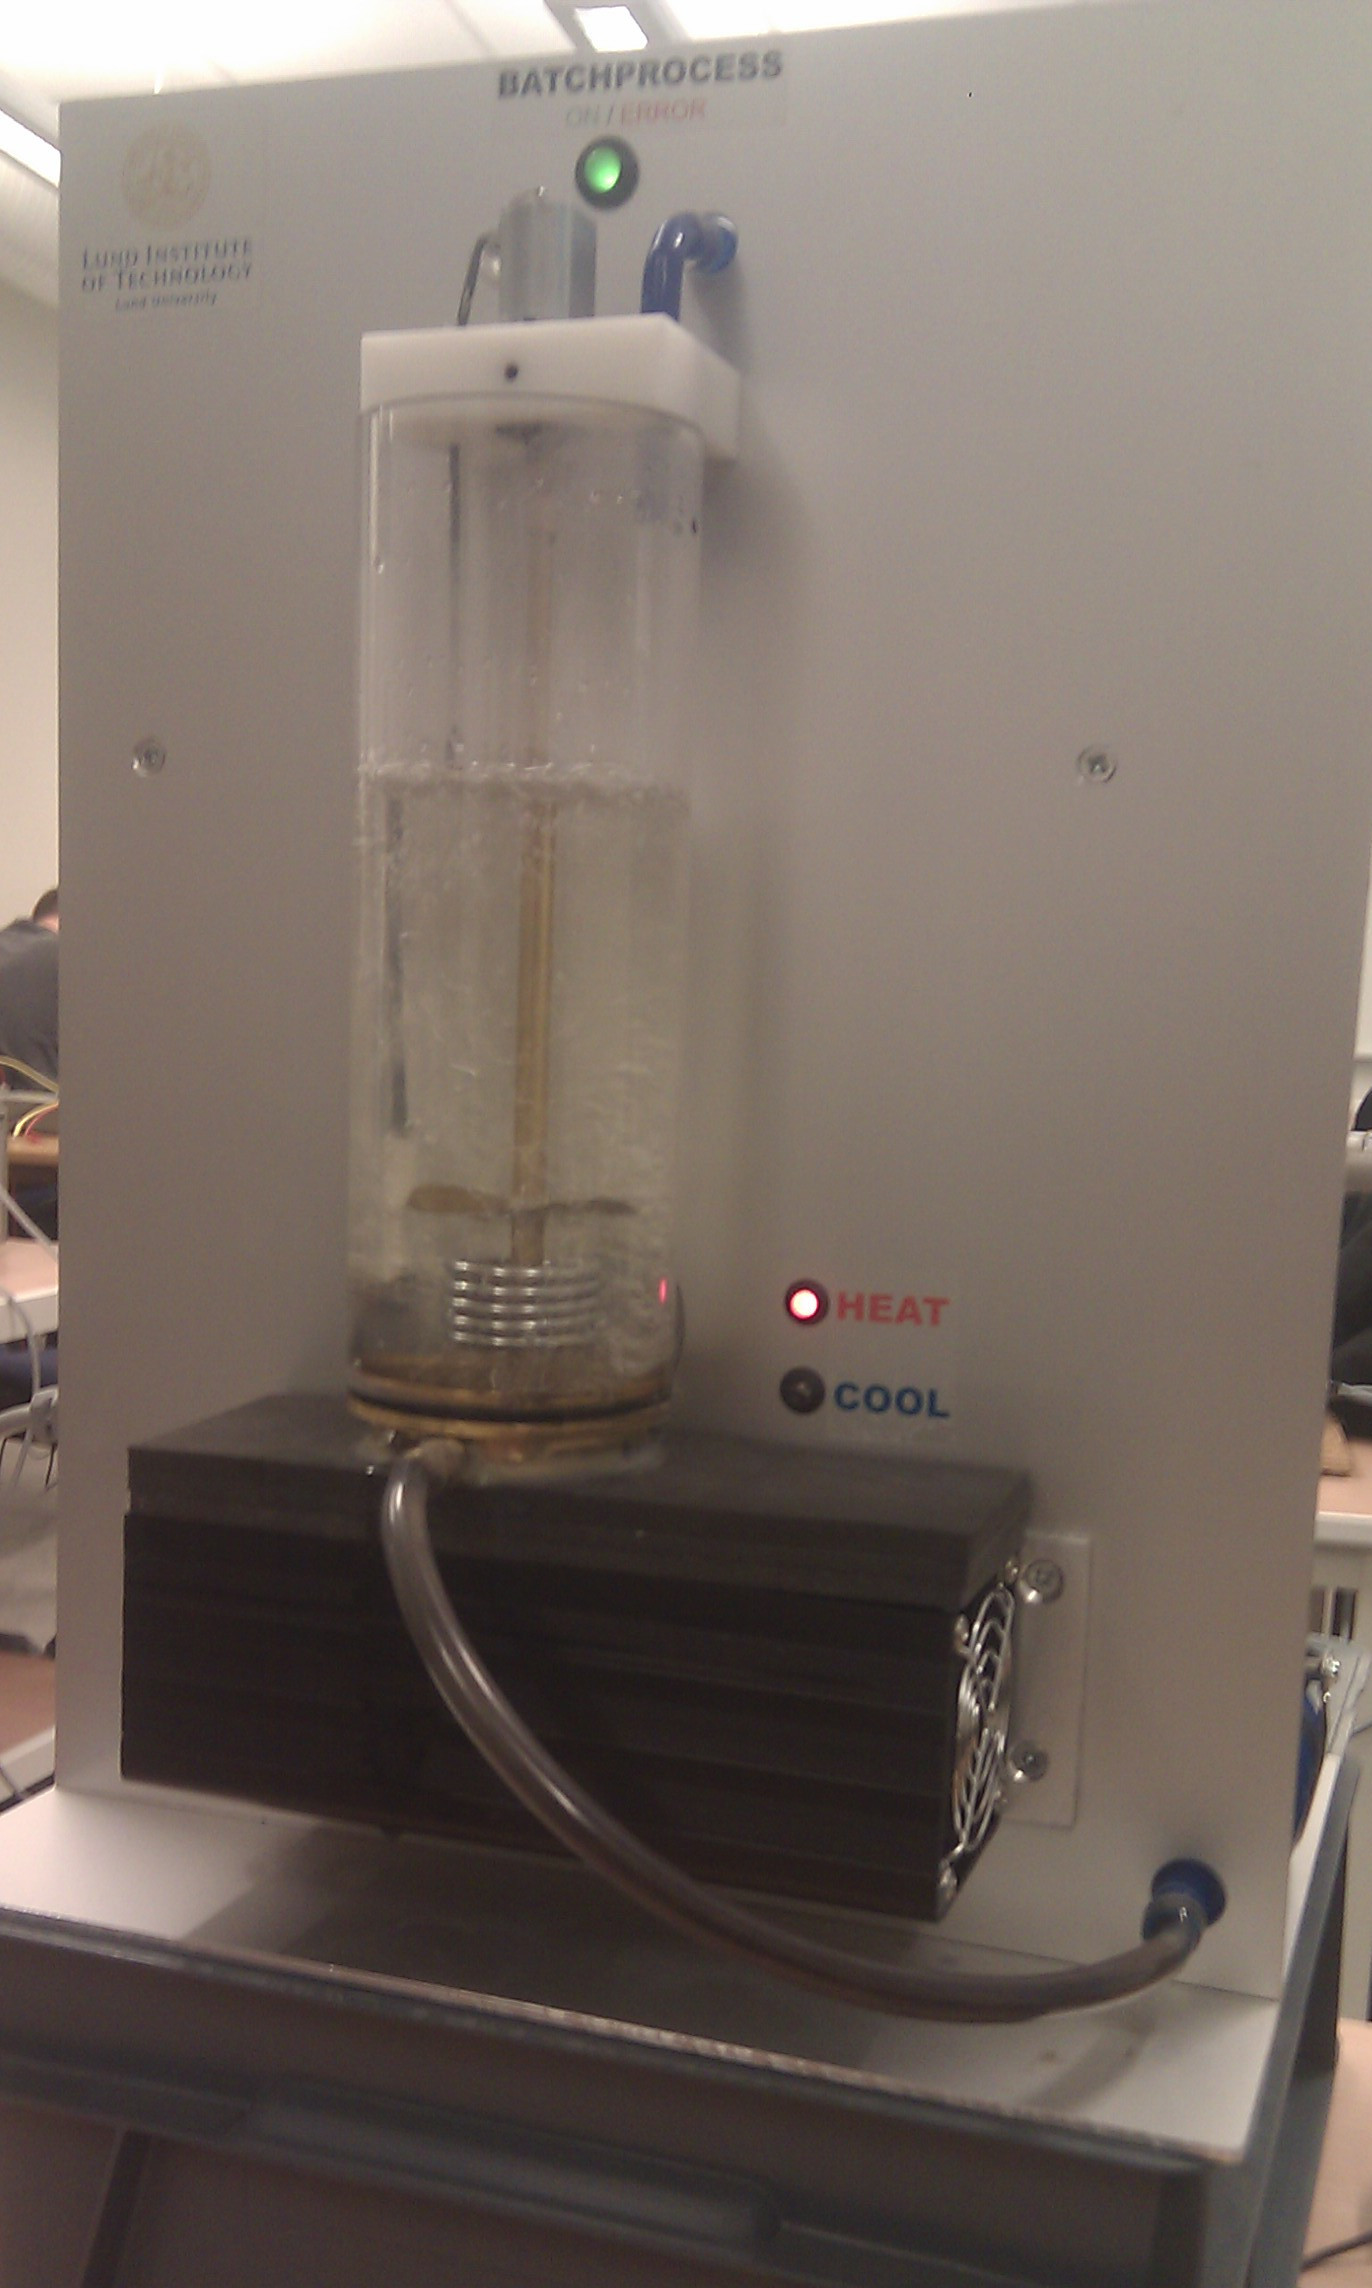
\includegraphics[width=0.7\textwidth]{batchprocess.jpg}
        \end{figure}

    \end{column}
\end{columns}
\end{frame}

%--- Slide 2 ---%
\begin{frame}{System structure}
\begin{columns}[T]
    \begin{column}{.55\textwidth}
        \begin{itemize}
            \item Server/Client that communicates though TCP/IP.
            \item Server is connected to the batchprocess.
            \item Clients receives measurement data from the server and sends control data to the server.
        \end{itemize}
    \end{column}
    \begin{column}{.45\textwidth}

        \begin{figure}[H]
           \centering
           	Graphic explaining overall structure.
  %         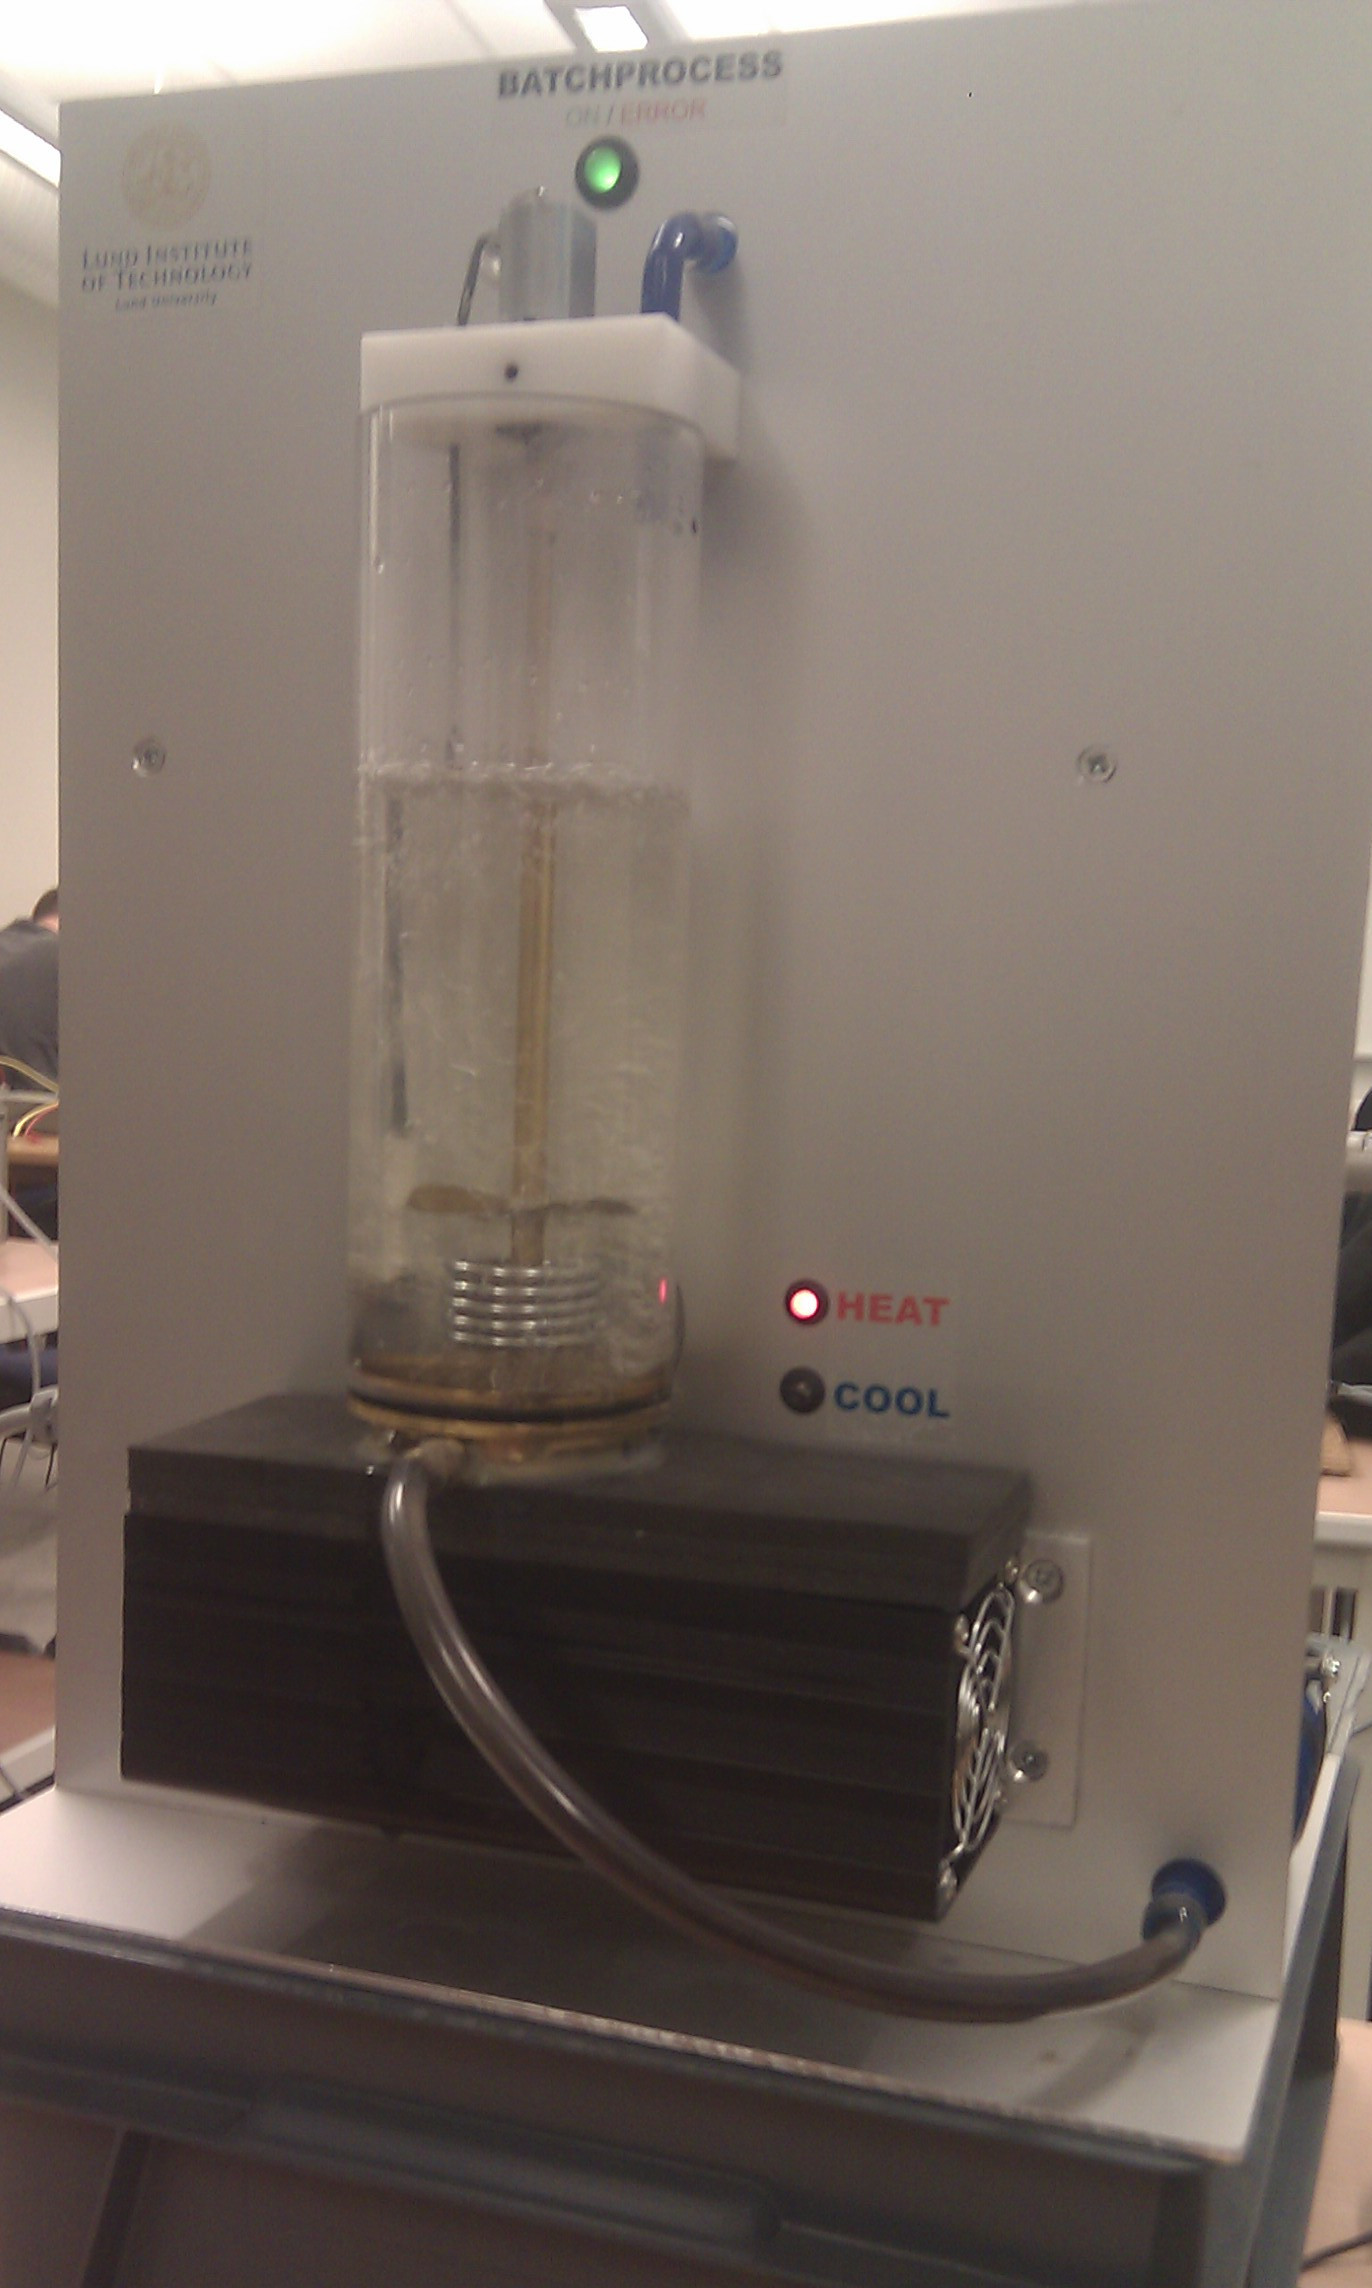
\includegraphics[width=0.7\textwidth]{batchprocess.jpg}
        \end{figure}

    \end{column}
\end{columns}
\end{frame}

%--- Slide 2 ---%
\begin{frame}{Server}
\begin{columns}[T]
    \begin{column}{.55\textwidth}
        \begin{itemize}
            \item Communicates with the batchprocess over a serial interface though a driver.
            \item Listens for connections from clients.
            \item Takes measurement data from the batchprocess and sends to the clients upon their request.
            	\item Receives control data from the clients and send it to the batchprocess.
        \end{itemize}
    \end{column}
    \begin{column}{.45\textwidth}

        \begin{figure}[H]
           \centering
           	Can haz pic plx?
  %         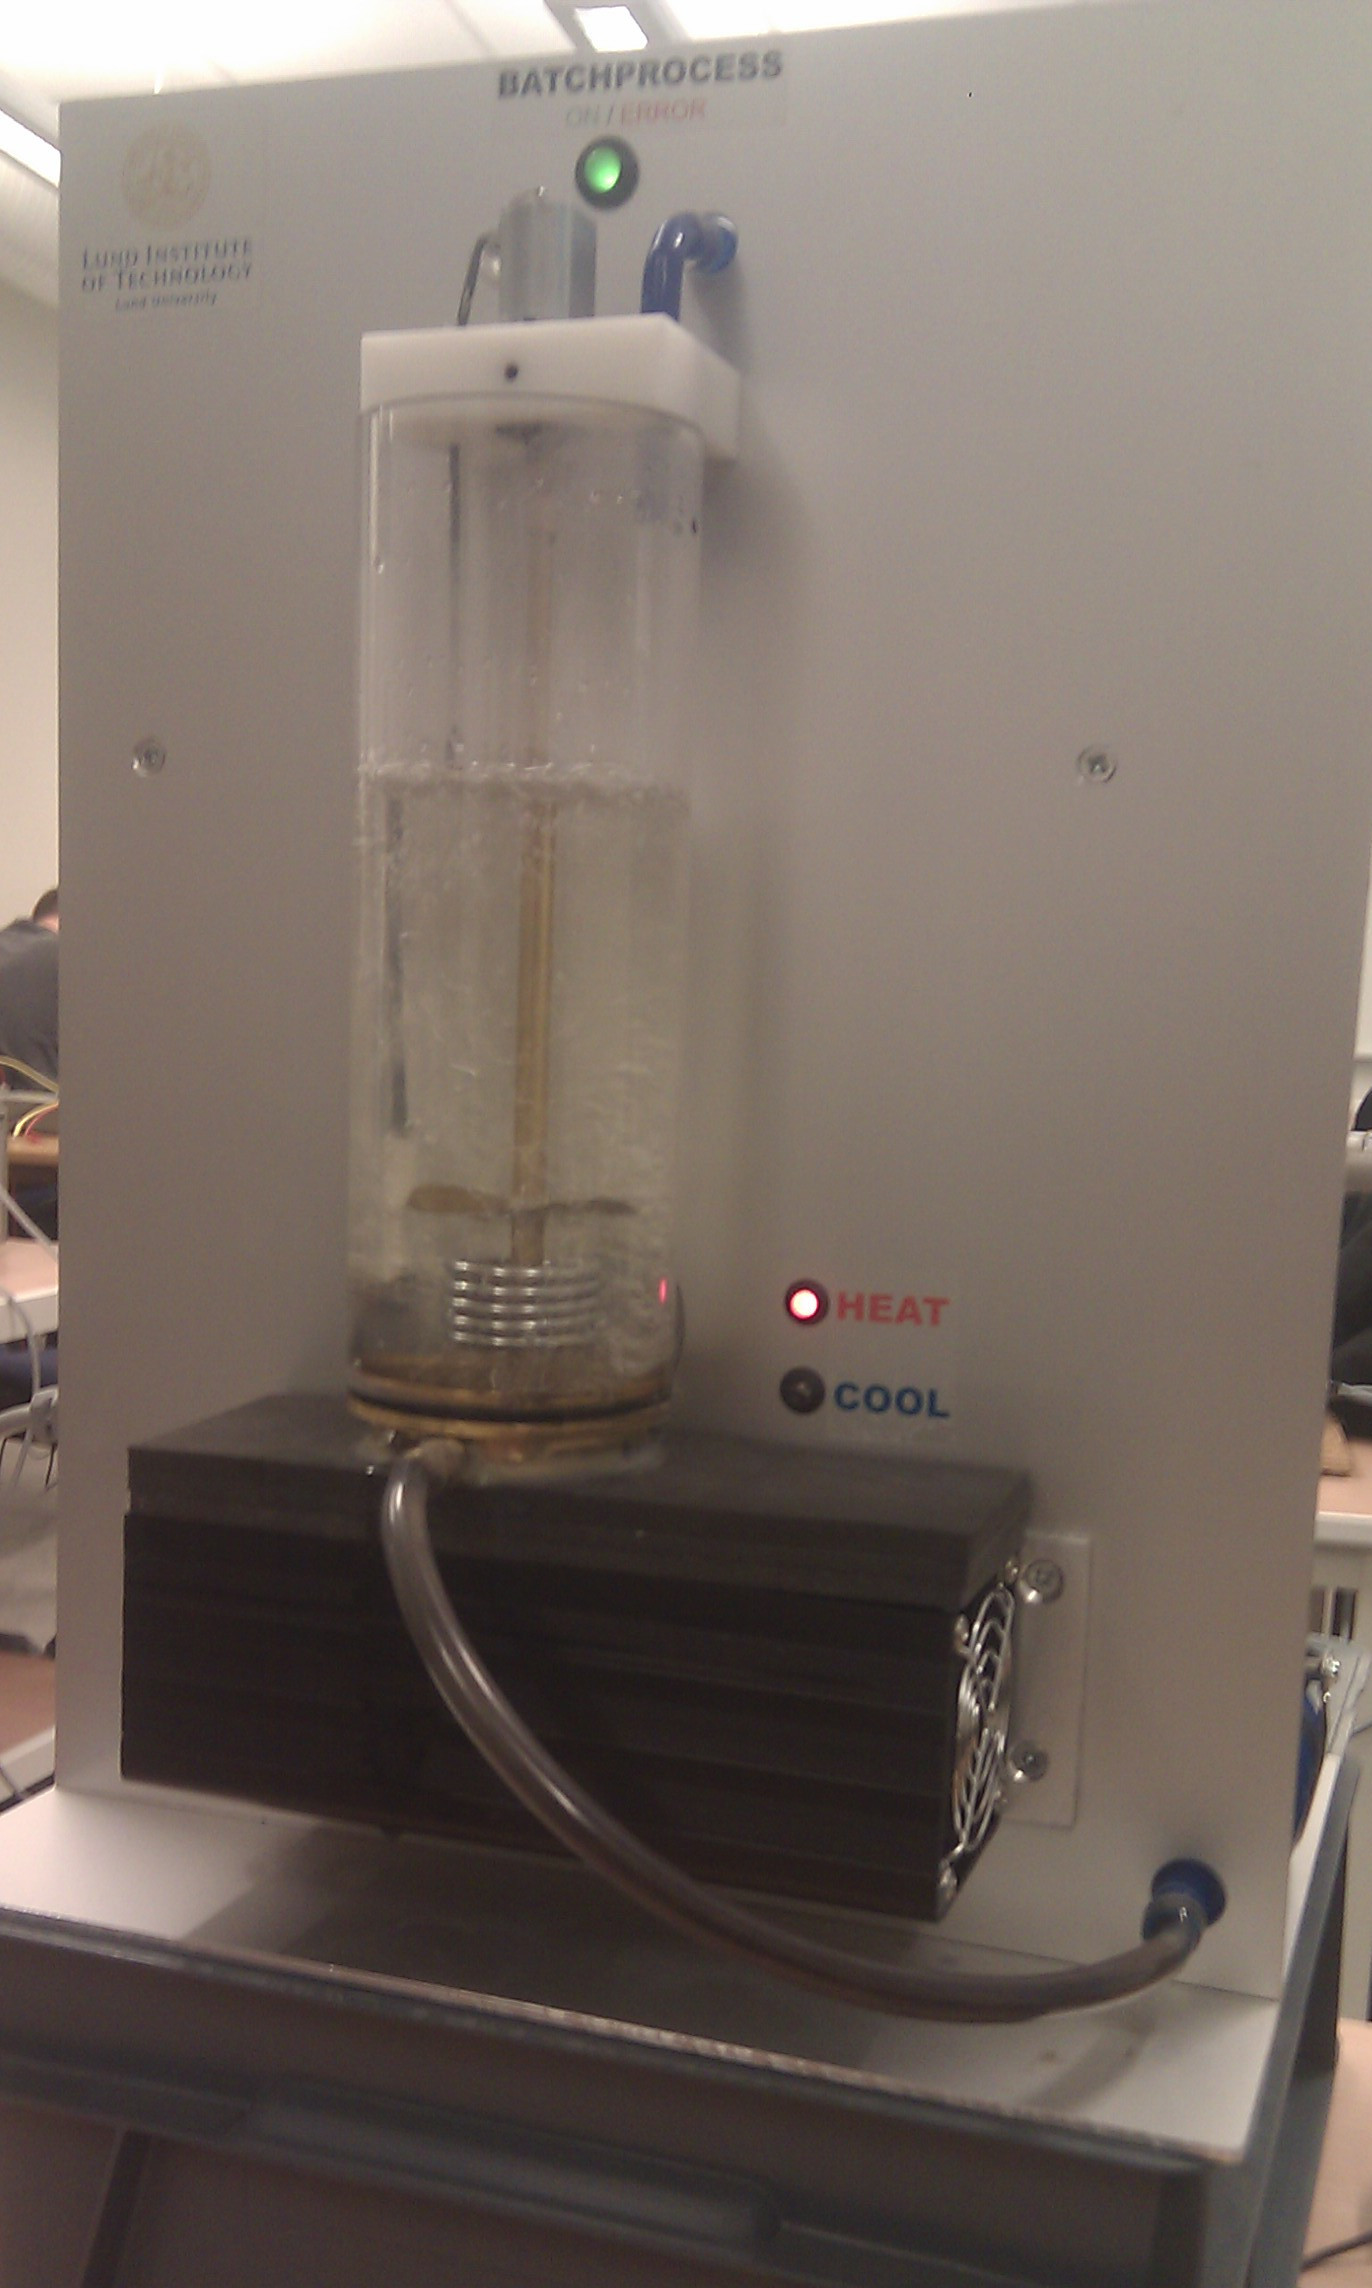
\includegraphics[width=0.7\textwidth]{batchprocess.jpg}
        \end{figure}

    \end{column}
\end{columns}
\end{frame}

%--- Slide 3 ---%
\begin{frame}{Driver}
\begin{columns}[T]
    \begin{column}{.55\textwidth}
        \begin{itemize}
            \item Driver for communicating with the batchprocess over a serial interface.
            \item Uses the Unix API termios.
            \item Uses standard C functions for I/O; read(2), write(3), open(2), close(2).
            \item Sends and receives data in chunks of 8 bits, the data is raw.   
        \end{itemize}
    \end{column}
    \end{columns}
\end{frame}

%--- Slide 4 ---%
\begin {frame}{Protocol - as seen in the batch tank source code}
/*
* +-+-+-+-+-+
* |0|cmd| chan |
* +-+-+-+-+-+
*
* 00 = bit clear, 01 = bit set, 10 = bit get, 11 = chan get
*
* +-+-+-+-+-+-+-+-+ +-+
* |1| bit8...bit2 | |0|bit| chan |
* +-+-+-+-+-+-+-+-+ +-+
*
* +-+-+-+-+-+-+-+-+ +-+-+-+-+-+-+-+
* |1|bit15...bit9 | |1| bit8...bit2 | |0|bit| chan |
* +-+-+-+-+-+-+-+-+ +-+-+-+-+-+-+-+
*
* ...
*
* +-+-+-+-+-+-+-+-+ +-+-+-+-+-+-+-+-+ +
* |1|bit31...bit30| |1|bit29...bit23| ... |0|bit| chan |
* +-+-+-+-+-+-+-+-+ +-+-+-+-+-+-+-+-+ +
*
*/
\end{frame}
%--- Slide 5 ---%
\begin{frame}{PID clients}
\begin{columns}[T]
    \begin{column}{.55\textwidth}
        \begin{itemize}
            \item A PID client receives measurement data from the server and calculates control data which then is sent to the server.
            
        \end{itemize}
    \end{column}
    \end{columns}
\end{frame}

%--- Slide 6 ---%
\begin{frame}{Plot client}
\begin{columns}[T]
    \begin{column}{.55\textwidth}
        \begin{itemize}
            \item A client that is a HTTP server.
            \item Receives measurement data and control data from the server.
            \item Listens for HTTP connections on port 8080.
            \item Serves a HTML, CSS and Javascript based plotting system.
            \item The plotting system sends AJAX GETs to the HTTP server which answers with the latest data.
            \item Plots multiple curves on multiple plots.
        \end{itemize}
    \end{column}
    \begin{column}{.45\textwidth}
        \begin{figure}[H]
           \centering
           	Plot pic.
  %         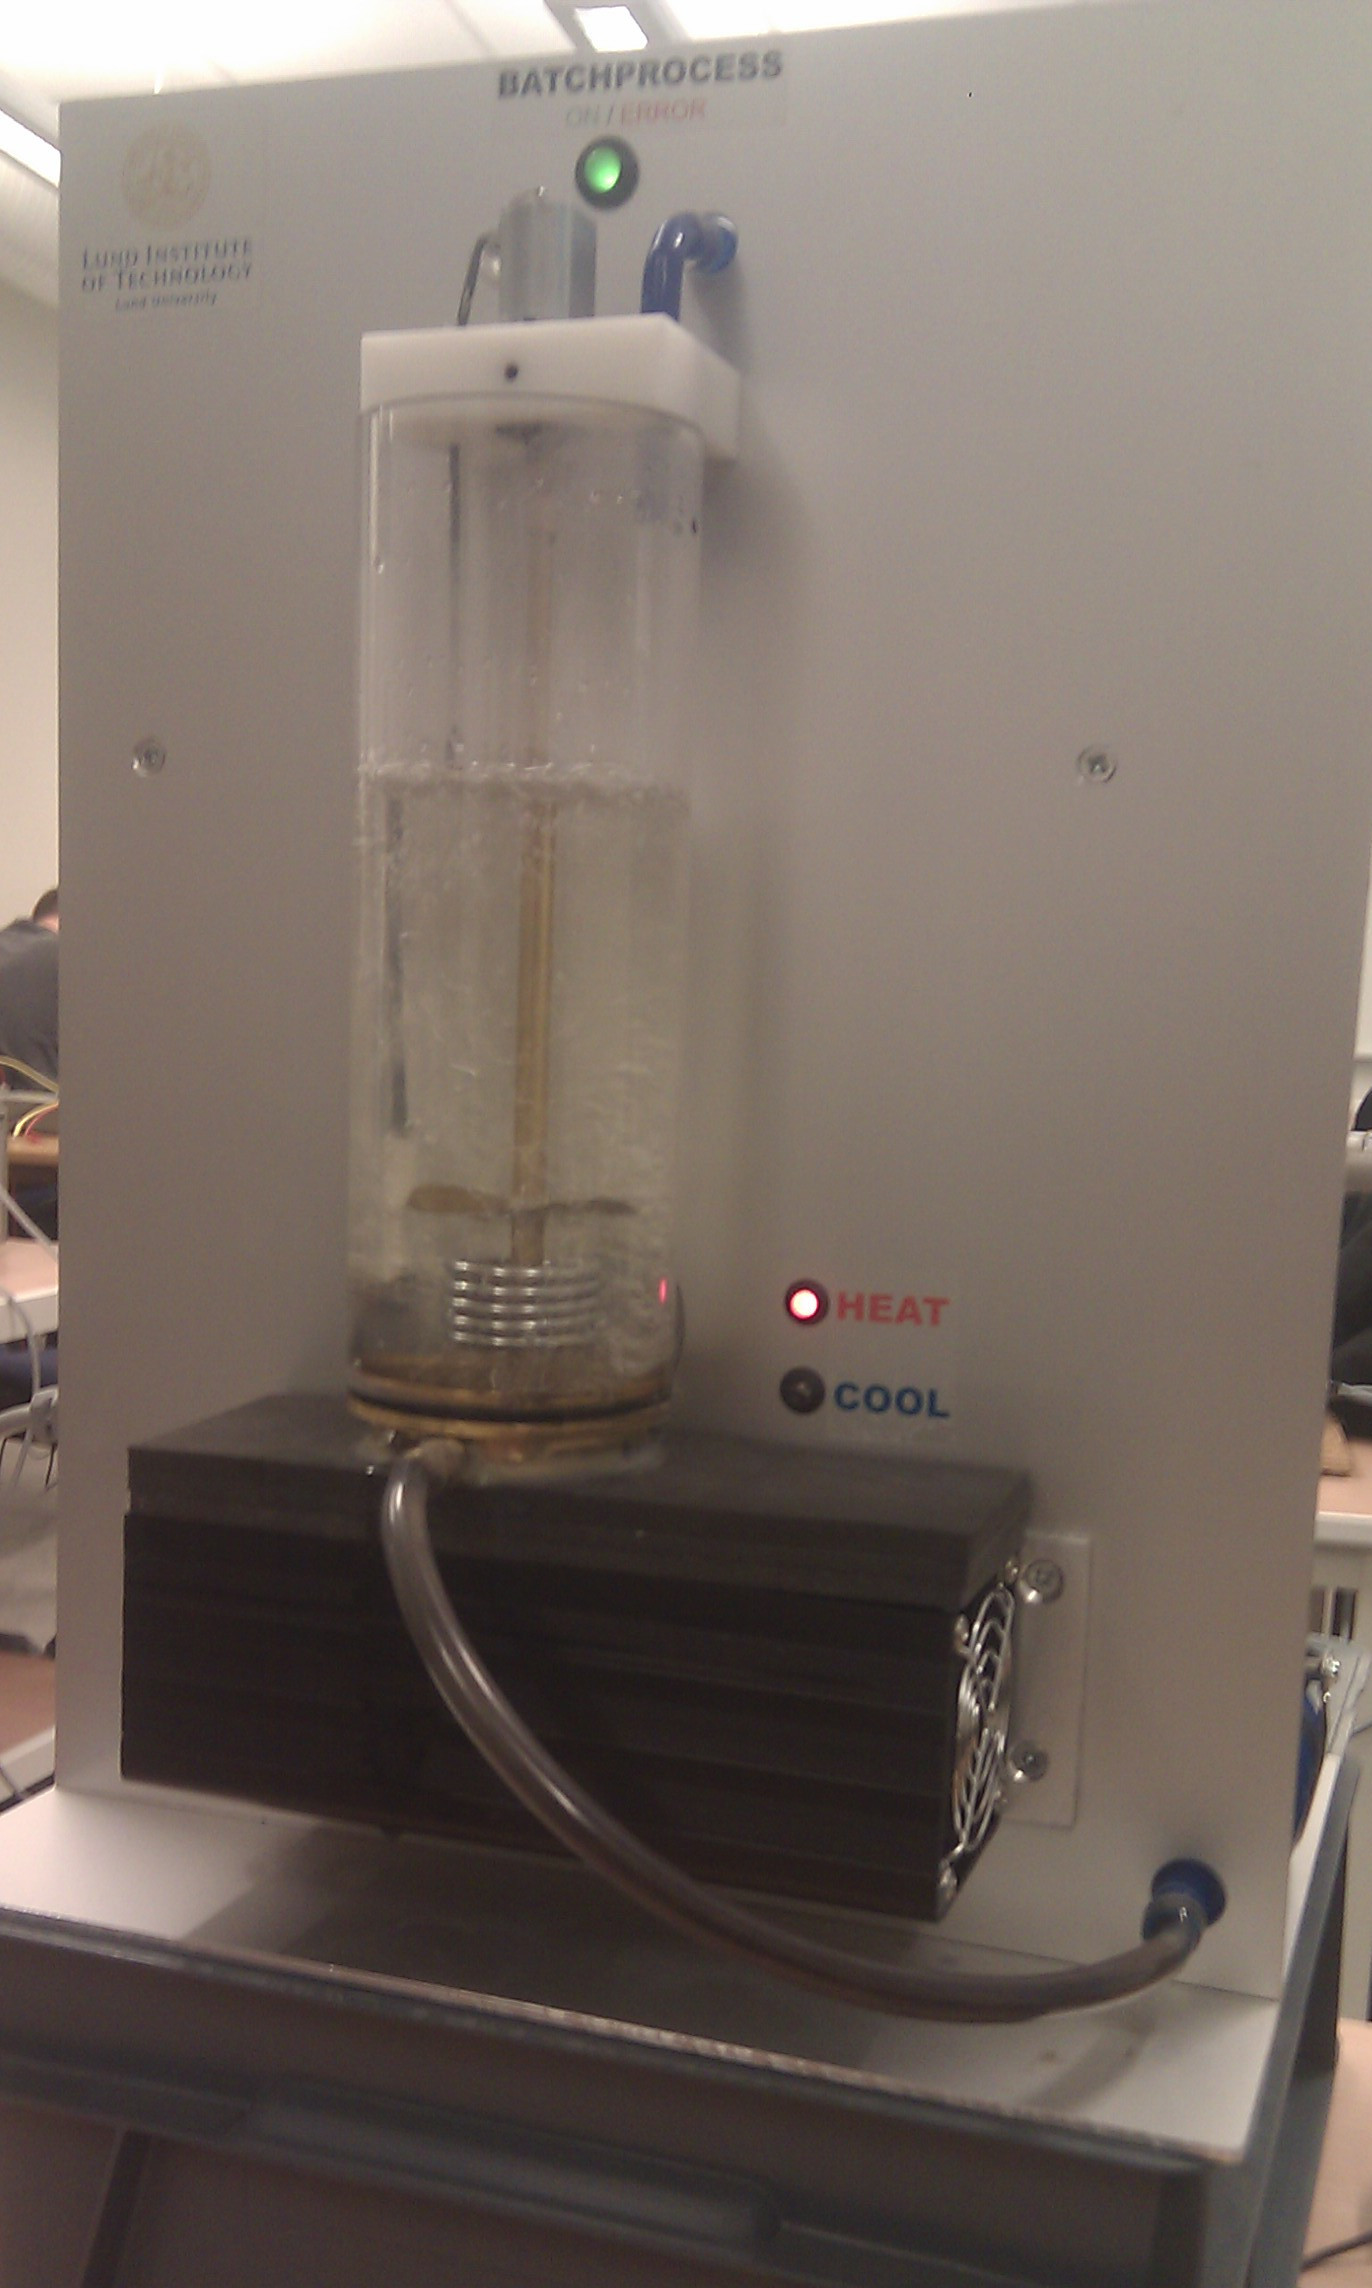
\includegraphics[width=0.7\textwidth]{batchprocess.jpg}
        \end{figure}
    \end{column}
    \end{columns}
\end{frame}

\end{document}